\chapter{Systementwurf}\label{ch:systementwurf}

Auf Grundlage der zuvor definierten Anforderungen wird in diesem Kapitel der Entwurf des Gesamtsystems beschrieben. Zunächst wird ein übergeordnetes Systemkonzept vorgestellt, das die zentralen Komponenten und deren Zusammenwirken darstellt. Anschließend werden die Funktionen den verfügbaren Hardwarekomponenten der Zielplattform zugeordnet und die mehrstufige KI-Verarbeitungskette von der Bilderfassung bis zur Klassifikation des dargestellten Fingeralphabetzeichens beschrieben. Ergänzend wird erläutert, wie das Klassifikationsmodell auf einem externen Rechner trainiert und anschließend auf die eingebettete Zielplattform übertragen wird. Dabei wird insbesondere betrachtet, wie eine übereinstimmende Verarbeitung der Eingabedaten in der Trainings- und Inferenzpipeline sichergestellt werden soll.

Der Systementwurf legt damit die grundlegende Architektur und die Schnittstellen zwischen den einzelnen Komponenten fest. Die konkrete technische Umsetzung, darunter die Konfiguration der Peripherie, die Speicherverwaltung sowie die Vor- und Nachverarbeitung der Modelldaten, wird im nachfolgenden Implementierungskapitel behandelt.

\section{Systemkonzept}\label{sec:systemkonzept}

Ausgehend von den zuvor definierten Anforderungen wurde ein Systemkonzept entwickelt, das die funktionalen Komponenten des Gesamtsystems und den zwischen ihnen stattfindenden Datenfluss beschreibt. Das Konzept stellt zunächst eine weitgehend von der konkreten Zielplattform unabhängige Betrachtung des Systems dar. Dadurch können die erforderlichen Verarbeitungsschritte festgelegt werden, bevor diese im Hardware- und Softwareentwurf konkreten Komponenten der Zielplattform zugeordnet werden. Das in Abbildung~\ref{fig:systemkonzept} dargestellte Blockdiagramm veranschaulicht den Datenfluss von der Aufnahme eines Kamerabildes bis zur Ausgabe des erkannten Fingeralphabetzeichens auf dem Display.

\begin{figure}[!htbp]
    \centering
    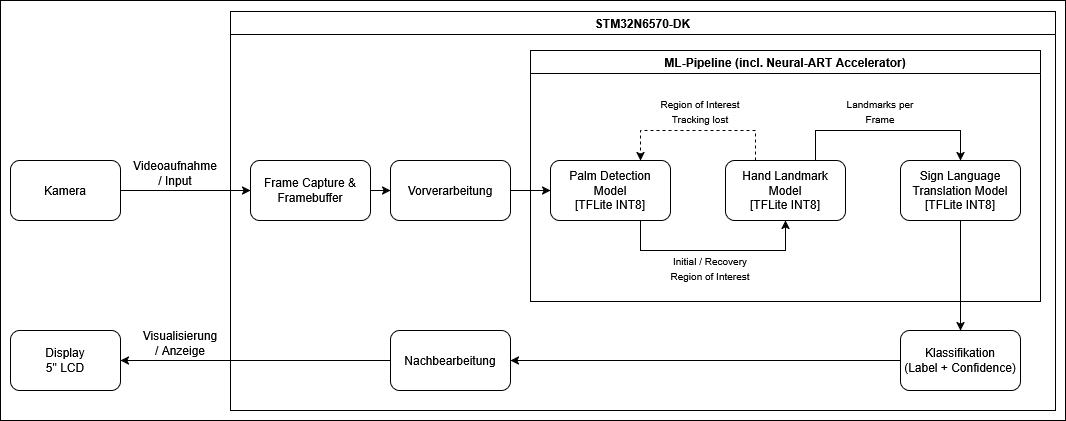
\includegraphics[width=\textwidth]{material/figures/Systemkonzept_erweitert.png}
    \caption{Blockdiagramm des Systemkonzepts}
    \label{fig:systemkonzept}
\end{figure}

Die Kamera erfasst kontinuierlich Bilddaten und überträgt diese an das System. Die aufgenommenen Bilder werden zunächst in einem Bildpuffer zwischengespeichert. Für die Handdetektion wird das Kamerabild auf die erforderliche Eingangsauflösung skaliert und anschließend der Verarbeitungskette bereitgestellt. Die Zwischenspeicherung entkoppelt die kontinuierliche Bildaufnahme von den nachfolgenden Verarbeitungsschritten, deren Ausführungsdauer abhängig vom aktuellen Zustand der KI-Verarbeitungskette variieren kann.

Innerhalb der Verarbeitungskette kommen drei aufeinander aufbauende neuronale Netze \linebreak zum Einsatz. Alternativ wäre eine unmittelbare Klassifikation des vollständigen Kamerabildes durch ein einzelnes Modell denkbar. Ein solcher Ansatz müsste jedoch gleichzeitig die Hand lokalisieren, deren Merkmale extrahieren und das dargestellte Zeichen klassifizieren. Die gewählte Aufteilung ermöglicht dagegen eine getrennte Entwicklung und Überprüfung der Handdetektion, Landmark-Erkennung und Zeichenklassifikation. Zudem verarbeitet das Klassifikationsmodell ausschließlich die Landmark-Koordinaten und benötigt dadurch keinen vollständigen Bildausschnitt als Eingabe. Nachteilig ist die höhere Komplexität der mehrstufigen Verarbeitungskette, da die einzelnen Komponenten und ihre Parameter aufeinander abgestimmt werden müssen. Dem steht jedoch der Vorteil gegenüber, für jede Verarbeitungsstufe ein spezialisiertes Modell einsetzen zu können, das gezielt für die jeweilige Aufgabe der Handdetektion, Landmark-Erkennung oder Zeichenklassifikation ausgelegt ist.

Im ersten Verarbeitungsschritt wird mithilfe des Handdetektionsmodells geprüft, ob sich eine Hand im Kamerabild befindet. Für eine erkannte Hand werden deren Position und räumliche Ausdehnung bestimmt. Aus diesen Informationen wird eine Region of Interest gebildet, die den für die weiteren Verarbeitungsschritte relevanten Bildbereich enthält. Durch die Beschränkung auf diesen Ausschnitt muss das nachfolgende Landmark-Modell nicht das vollständige Kamerabild verarbeiten. Gleichzeitig setzt dieses Vorgehen voraus, dass die Hand zunächst zuverlässig lokalisiert wird.

Das zweite Modell bestimmt innerhalb der Region of Interest die charakteristischen Handlandmarks. Die ermittelten Koordinaten werden anschließend nachverarbeitet und in eine für das Klassifikationsmodell geeignete Form überführt. Hierzu gehören insbesondere die Anpassung des Datenformats und die Normalisierung der Landmark-Koordinaten. Die Verwendung von Landmarks reduziert die Eingabedaten des Klassifikationsmodells auf die geometrische Anordnung der Handpunkte. Bildmerkmale wie Hintergrund, Hautfarbe und Texturen werden dadurch nicht unmittelbar zur Klassifikation herangezogen. Die Erkennungsleistung hängt jedoch entsprechend stark von der Genauigkeit und Stabilität der Landmark-Erkennung ab. Aus den erkannten Landmarks wird außerdem die Region of Interest für das folgende Kamerabild aktualisiert. Dadurch muss das Handdetektionsmodell nicht in jedem Verarbeitungsdurchlauf erneut ausgeführt werden. Gegenüber einer wiederholten vollständigen Handdetektion reduziert dieser Ansatz den Rechenaufwand und ermöglicht eine kontinuierliche Verfolgung der Hand. \cite[S. 4]{zhangMediaPipeHandsOndevice2020} Gleichzeitig können sich Fehler bei der Aktualisierung der Region über mehrere Bilder fortsetzen. Wird keine gültige Landmark-Ausgabe mehr erzeugt, wird das Tracking daher zurückgesetzt und erneut die Handdetektion ausgeführt.

Das dritte Modell klassifiziert die aufbereiteten Handlandmarks und ordnet die dargestellte Handform einer der unterstützten Zeichenklassen zu. Das Klassifikationsergebnis wird gemeinsam mit dem Kamerabild auf dem Display ausgegeben. Liegt keine gültige Hand- oder Landmark-Erkennung vor, wird kein Fingeralphabetzeichen ausgegeben. Für nicht eindeutige Zeichen ist zusätzlich die Klasse \texttt{NONE} vorgesehen. Die Verarbeitungskette wird zyklisch ausgeführt, sodass Änderungen der Handposition und des dargestellten Handzeichens fortlaufend berücksichtigt werden können. Eine übergeordnete Ablaufsteuerung koordiniert dabei die Bildaufnahme, die Ausführung der Modelle, die Vor- und Nachverarbeitung sowie die Aktualisierung der grafischen Ausgabe.

\section{Hardwarekonzept}\label{sec:hardwarekonzept}

Das Hardwarekonzept überführt die im Systemkonzept festgelegten Funktionen auf die Komponenten der eingebetteten Zielplattform. Als zentrale Verarbeitungseinheit wird das STM32-N6570 Discovery Kit verwendet. Neben dem Mikrocontroller umfasst der Hardwareaufbau das Kameramodul MB1854B mit dem Bildsensor IMX335, das Displaymodul MB1860B sowie die auf dem Board vorhandenen externen Speicher \cite{STM32N6570DKProductSTMicroelectronics}.

Die Auswahl des STM32N6570 Discovery Kits dient der experimentellen Untersuchung, ob die vollständige Verarbeitungskette auf einer mikrocontrollerbasierten Plattform umgesetzt werden kann. Alternativ wäre der Einsatz eines Einplatinencomputers oder einer Plattform mit einer leistungsfähigeren GPU denkbar. Eine solche Plattform würde die Modellausführung und Bildverarbeitung vereinfachen, entspräche jedoch nicht dem in dieser Arbeit untersuchten Ansatz eines ressourcenbeschränkten eingebetteten Systems. Als Alternative innerhalb derselben Mikrocontrollerfamilie wurde das NUCLEO-N657X0-Q betrachtet. Dieses verwendet ebenfalls einen STM32N657 und stellt damit grundsätzlich dieselben zentralen Verarbeitungsfunktionen einschließlich des Neural-ART Accelerators bereit. Das Board besitzt jedoch kein integriertes Display und wird ohne angeschlossenes Kameramodul ausgeliefert. Zwar steht ein FPC-Anschluss für ein Kameramodul zur Verfügung, Kamera und Display müssten jedoch zusätzlich ausgewählt, angeschlossen und in das System integriert werden \cite{STMicroelectronicsNUCLEON657X0Q}.

Das STM32N6570 Discovery Kit enthält dagegen bereits ein Kameramodul, ein LCD-Modul sowie externe PSRAM- und NOR-Flash-Speicher. Damit stellt es die für die vorgesehene Kamera- und KI-Verarbeitung benötigten Komponenten in einer gemeinsamen Entwicklungsplattform bereit und reduziert den zusätzlichen Integrationsaufwand. STMicroelectronics präsentiert die STM32N6-Plattform zudem ausdrücklich für Edge-AI- und Computer-Vision- \linebreak Anwendungen unter Verwendung des Neural-ART Accelerators, der MIPI-CSI-Schnittstelle und der integrierten Bildverarbeitung. Das Discovery Kit eignet sich daher besonders für die prototypische Untersuchung der in dieser Arbeit entwickelten Verarbeitungskette \cite{STM32N6570DKProductSTMicroelectronics}.

Die Kameradaten werden über die CSI-Schnittstelle empfangen und mithilfe der Digital Camera Interface Pixel Pipeline verarbeitet. Die DCMIPP übernimmt hardwarenahe Verarbeitungsschritte wie die Umwandlung des Bildformats, den Bildzuschnitt und die Skalierung auf die benötigten Auflösungen. Alternativ könnten diese Operationen nach der Speicherung des Kamerabildes durch den Hauptprozessor ausgeführt werden. Dies würde jedoch zusätzliche CPU-Rechenzeit und Zugriffe auf die großformatigen Bilddaten erfordern. Die DCMIPP ermöglicht dagegen eine Aufbereitung während des Kameradatenflusses, bevor die erzeugten Bilder in den Zielspeicher geschrieben werden. Ihre Verwendung beschränkt die Verarbeitung allerdings auf die von der Hardware unterstützten Operationen und Konfigurationsmöglichkeiten.

Für die Ausführung der unterstützten Modelloperationen wird der integrierte Neural-ART Accelerator eingesetzt. Eine ausschließliche Ausführung auf dem Hauptprozessor wäre grundsätzlich möglich, würde jedoch dessen Rechenzeit stark beanspruchen und die erreichbare Verarbeitungsgeschwindigkeit begrenzen. Der spezialisierte Beschleuniger übernimmt daher die rechenintensiven Operationen der neuronalen Netze. Die grafische Ausgabe erfolgt über den LCD-TFT Display Controller. Dieser liest die darzustellenden Bilddaten kontinuierlich aus den zugeordneten Speicherbereichen und überträgt sie an das angeschlossene Display. Gegenüber einer softwareseitigen Übertragung jedes einzelnen Bildes entlastet der LTDC den Hauptprozessor von der kontinuierlichen Displayaktualisierung.

\section{KI-Verarbeitungskette}\label{sec:ki-verarbeitungskette}

Die KI-Verarbeitungskette besteht aus drei aufeinander aufbauenden Modellen zur Handdetektion, Handlandmark-Erkennung und Klassifikation des dargestellten Fingeralphabetzeichens. Abbildung \ref{fig:ml-sequence} zeigt die einzelnen Verarbeitungsschitte sowie die beiden durch die DCMIPP bereitgestellten Bildpfade.

\begin{figure}[!htbp]
    \centering
    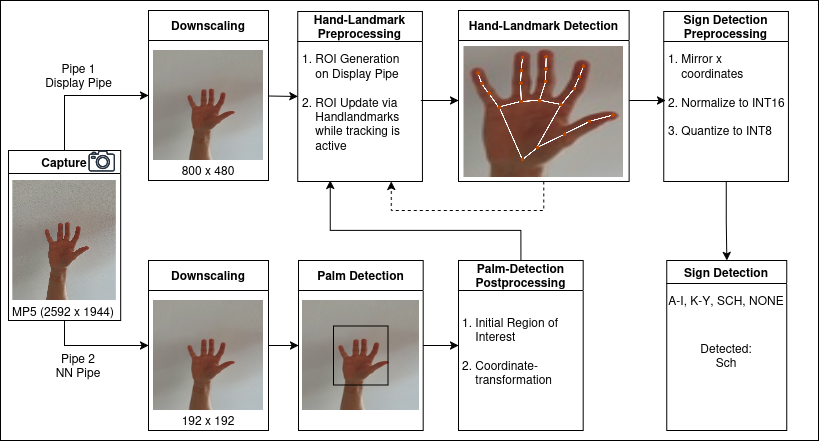
\includegraphics[width=\textwidth]{material/figures/ML_sequence_v3.png}
    \caption{KI-Verarbeitungskette zur Erkennung der Fingeralphabetzeichen}
    \label{fig:ml-sequence}
\end{figure}

Ausgangspunkt der Verarbeitungskette ist das von der Kamera aufgenommene Bild mit einer Auflösung von 2592×1944 Pixeln. Die DCMIPP stellt den Kameradatenstrom parallel über zwei getrennte Verarbeitungspfade bereit. Pipe 1 erzeugt ein Bild mit einer Auflösung von 800 × 480 Pixeln, das für die Displayausgabe und als Ausgangsbild der Handlandmark-Erkennung verwendet wird. Pipe 2 erzeugt parallel dazu ein Bild mit einer Auflösung von 192×192 Pixeln für die Handdetektion. Das Handdetektionsmodell verarbeitet das von Pipe 2 bereitgestellte Bild und ermittelt die Position einer vorhandenen Hand. Im Rahmen der Nachverarbeitung wird aus dem Modellergebnis eine initiale Region of Interest bestimmt. Da die Handdetektion und die Landmark-Erkennung unterschiedliche Bildpfade verwenden, wird die Region of Interest anschließend in das Koordinatensystem des von Pipe 1 erzeugten Bildes übertragen. Auf Grundlage der transformierten Region of Interest wird aus dem Bild von Pipe 1 ein Ausschnitt mit einer Auflösung von 224×224 Pixeln erzeugt. Dieser Ausschnitt wird für das Handlandmark-Modell aufbereitet und anschließend an das Modell übergeben. Das Handlandmark-Modell bestimmt die Positionen der charakteristischen Landmark-Punkte innerhalb der Handregion.

Nach einer erfolgreichen Landmark-Erkennung wird die Region of Interest anhand der Modellausgabe aktualisiert. Für die Verarbeitung des folgenden Kamerabildes wird dadurch nicht erneut die gesamte Handdetektion ausgeführt. Stattdessen wird aus dem nächsten Bild von Pipe 1 unmittelbar eine neue Landmark-Eingabe auf Grundlage der aktualisierten Region erzeugt. Dieser Rückkopplungspfad bildet das Landmark-Tracking. Kann das Handlandmark-Modell über mehrere aufeinanderfolgende Bilder keine gültige Hand mehr bestimmen, wird das Tracking beendet. Das System wechselt daraufhin zurück zur Handdetektion, um erneut eine initiale Region of Interest im vollständigen Bild zu bestimmen. Die Handdetektion und das Landmark-Tracking bilden somit zwei aufeinander abgestimmte Zustände der Verarbeitungskette.

Für die anschließende Zeichenklassifikation werden ausschließlich die ermittelten Landmark-Koordinaten verwendet. Vor der Übergabe an das Klassifikationsmodell werden diese in eine einheitliche Darstellung überführt und an das erforderliche Eingabeformat angepasst. Dazu gehören die Berücksichtigung der erkannten Händigkeit, die Normalisierung der Koordinaten und deren Überführung in das vom quantisierten Klassifikationsmodell verwendete Zahlenformat. Die konkrete Berechnung dieser Schritte wird im Implementierungskapitel beschrieben.

Das Klassifikationsmodell ordnet die aufbereiteten Landmark-Koordinaten einer der für den Prototyp festgelegten Zeichenklassen zu. Zusätzlich wird die Klasse NONE berücksichtigt, wenn keine der unterstützten Handformen vorliegt. Das ermittelte Klassifikationsergebnis wird anschließend an die grafische Ausgabe übergeben und auf dem Display dargestellt.

\section{Trainings- und Übertragungskonzept}\label{sec:trainingskonzept}

Das Training des Klassifikationsmodells erfolgt auf einem externen Entwicklungsrechner, da die Zielplattform weder für die rechenintensive Modelloptimierung noch für die Verwaltung des vollständigen Trainingsdatensatzes vorgesehen ist. Als Trainingshardware wird ein Rechner mit einem \texttt{Intel Core i7-12700KF} Prozessor, \texttt{32 GB DDR5} Arbeitsspeicher und einer \texttt{Geforce RTX 4060 TI 16 GB} Grafikkarte verwendet. Auf dem Rechner kommt \texttt{Linux \linebreak CashyOS} \cite{CachyOS} als Betriebssystem zum Einsatz. Die konkrete Hardwareausstattung beeinflusst dabei hauptsächlich die Trainingsdauer, nicht jedoch die anschließend verwendete Modellarchitektur. Die Softwareumgebung basiert auf Python sowie TensorFlow und Keras. TensorFlow stellt die grundlegenden Funktionen für die Entwicklung und Ausführung neuronaler Netze bereit, während Keras als übergeordnete Schnittstelle für die Definition, das Training und die Auswertung des Klassifikationsmodells verwendet wird \cite{TensorFlow,Keras}. Die genauen Versionen sind in einer \texttt{requirements.txt} Datei festgehalten.

Die Handdetektion und das Handlandmark-Modell werden im Rahmen dieser Arbeit nicht erneut trainiert. Sie bilden feste Bestandteile der Verarbeitungskette und dienen dazu, aus den aufgenommenen Kamerabildern die Eingabemerkmale für das Klassifikationsmodell zu erzeugen. Für die Erstellung der Trainingsdaten wird auf dem Entwicklungsrechner eine Referenzpipeline eingesetzt. Diese verwendet dieselben Ausgangsmodelle für die Handdetektion und Landmark-Erkennung, die anschließend für die eingebettete Zielplattform konvertiert werden. Aus den ermittelten Handlandmarks werden die für die Zeichenklassifikation benötigten Merkmale gebildet. Dazu gehören die Auswahl und Reihenfolge der Koordinaten, die Spiegelung der horizontalen Koordinaten, die Bildung handgelenkrelativer Werte sowie die Zuordnung zur linken beziehungsweise rechten Hand. Das Klassifikationsmodell wird auf Grundlage dieser Merkmalsdarstellung trainiert und anschließend in ein quantisiertes TensorFlow-Lite-Modell überführt.

Die Konsistenz zwischen Trainings- und Inferenzpipeline wird auf mehreren Ebenen berücksichtigt. Für beide Plattformen werden dieselbe Landmark-Reihenfolge, dieselbe Merkmalsanordnung und dieselben Koordinatentransformationen verwendet. Darüber hinaus werden die Eingangsauflösungen, Farbkanalreihenfolgen und Region-of-Interest-Transformationen eindeutig festgelegt. Die auf dem Mikrocontroller implementierte Vor- und Nachverarbeitung bildet diese Festlegungen entsprechend nach. Die Modelle werden mithilfe von ST Edge AI Core in ein für den Neural-ART Accelerator ausführbares Format konvertiert. Dabei findet kein erneutes Training statt. Die zuvor ermittelten Modellgewichte werden lediglich quantisiert beziehungsweise in eine für die Zielplattform geeignete Darstellung überführt. Aufgrund der Quantisierung und der unterschiedlichen numerischen Ausführung ist keine bitgenaue Übereinstimmung zwischen Entwicklungsrechner und Zielplattform zu erwarten.

\section{Speicher- und Datenflusskonzept}\label{sec:speicher-datenfluss}

Die im Gesamtsystem anfallenden Daten unterscheiden sich deutlich hinsichtlich ihres Umfangs, ihrer Lebensdauer und ihrer Verwendung. Aus diesem Grund werden die Kamerabilder, Modellgewichte, Modellein- und -ausgaben sowie Steuerungsdaten auf unterschiedliche Speicherbereiche der Zielplattform verteilt. Abbildung \ref{fig:datenfluss} zeigt die vorgesehene Zuordnung der Daten zu den verfügbaren Speichern sowie den Datenfluss zwischen den beteiligten Hardware- und Softwarekomponenten.

\begin{figure}[!htbp]
    \centering
    
\includegraphics[width=\textwidth]{material/figures/qC App Data Flow Diagram.drawio.png}
    \caption{Speicher- und Datenflusskonzept des Gesamtsystems}
    \label{fig:datenfluss}
\end{figure}

Die großformatigen Kamera- und Displaydaten werden im externen PSRAM gespeichert. Für das von Pipe 1 erzeugte Displaybild stehen vier Hintergrundbildpuffer zur Verfügung. Die mehreren Puffer ermöglichen es, die Bilderfassung, die KI-Verarbeitung, das Einzeichnen der Erkennungsergebnisse und die Displayausgabe auf voneinander getrennten Bildständen durchzuführen. Die Hintergrundbildpuffer werden durch den LTDC als Layer 1 ausgegeben. Zusätzlich greift der Hauptprozessor auf diese Puffer zu, um den Bildausschnitt für das Handlandmark-Modell zu erzeugen und die Region of Interest sowie die Handlandmarks direkt in das Displaybild einzuzeichnen.

Für die grafische Benutzeroberfläche stehen zwei separate Vordergrundpuffer im PSRAM zur Verfügung. Sie werden dem zweiten Layer des LTDC zugeordnet und enthalten unter anderem Bedienelemente, Statusinformationen und die Ausgabe des erkannten Fingeralphabetzeichens. Die doppelte Pufferung ermöglicht es, einen neuen Inhalt vorzubereiten, während der andere Puffer durch den LTDC ausgegeben wird. Der LTDC kombiniert den Hintergrund aus Layer 1 mit dem teilweise transparenten Vordergrund aus Layer 2 zur endgültigen Displayausgabe.

Pipe 2 erzeugt die auf 192×192 Pixel verkleinerten Eingabebilder für die Handdetektion. Diese werden abwechselnd in zwei weiteren Puffern in der externen PSRAM gespeichert. Während ein Puffer durch die DCMIPP beschrieben wird, kann der zuvor fertiggestellte Puffer für die Handdetektion bereitgestellt werden.

Die Gewichte der drei neuronalen Netze werden im externen NOR-Flash abgelegt. Für die Handdetektion, die Handlandmark-Erkennung und die Zeichenklassifikation sind jeweils getrennte Modelldaten vorgesehen. Da die Modellgewichte während des regulären Betriebs nicht verändert werden, können sie dauerhaft im nichtflüchtigen Speicher verbleiben. Für die Ausführung der neuronalen Netze werden NPU-erreichbare Arbeitsspeicherbereiche verwendet. Jedes Modell benötigt einen Eingabepuffer, Aktivierungspuffer für die während der Inferenz entstehenden Zwischenergebnisse und einen Ausgabepuffer. Diese Daten werden nur für die Modellausführung benötigt und daher nicht dauerhaft gespeichert.

Die Modellausgaben werden durch den Hauptprozessor nachverarbeitet. Das Ergebnis der Handdetektion wird zur Bestimmung der initialen Region of Interest verwendet. Mithilfe dieser Region wird aus einem Hintergrundbildpuffer ein Ausschnitt für das Handlandmark-Modell erzeugt und in dessen Eingabepuffer übertragen. Die Ausgaben des Landmark-Modells werden zur Aktualisierung der Region of Interest, zur Darstellung der Landmark-Punkte und als Grundlage für die Zeichenklassifikation verwendet.

Nach der Aufbereitung werden die Landmark-Daten in den Eingabepuffer des Klassifikationsmodells übertragen. Dessen Ausgabe wird durch den Hauptprozessor in ein darstellbares Klassifikationsergebnis überführt und im dafür vorgesehenen Bereich im PSRAM abgelegt. Die Benutzeroberfläche greift auf diese Daten zu und übernimmt das Ergebnis in den Vordergrundpuffer.

Kleinere Steuerungs- und Zustandsdaten verbleiben im internen SRAM des Mikrocontrollers. Dazu gehören unter anderem der aktuelle Zustand der KI-Verarbeitungskette, die Region of Interest, die Landmark-Koordinaten, Zählerstände und Verwaltungsinformationen der Ablaufsteuerung.

\begin{longtable}[H]{|p{0.3\textwidth}|p{0.6\textwidth}|}
    \hline
    \textbf{Speicherbereich} & \textbf{Gespeicherte Daten} \\
    \hline
    \endfirsthead
    \hline
    \textbf{Speicherbereich} & \textbf{Gespeicherte Daten} \\
    \hline
    \endhead
    \hline
    \multicolumn{2}{r}{\texttt{Fortsetzung auf nächster Seite}} \\
    \endfoot
    \caption{Zuordnung der Systemdaten zu den Speicherbereichen}
    \label{tab:speicherzuordnung} \\
    \endlastfoot
    Externer PSRAM & Displaypuffer, Eingabebilder der Handdetektion \\
    \hline
    Externer NOR-Flash & Modellgewichte aller Modelle \\
    \hline
    NPU-erreichbarer Arbeits-speicher (AXI-RAM) & Eingabe-, Aktivierungs- und Ausgabepuffer der neuronalen Netze \\
    \hline
    Interner SRAM & Steuerungsdaten, Zustandsinformationen, Landmark-Daten und Klassifikationsergebnisse \\
    \hline
\end{longtable}

\section{Ablauf vom Kamerabild bis zum Erkennungsergebnis}\label{sec:ablauft}

In den vorherigen Abschnitten wurden zunächst die Komponenten des Gesamtsystems, deren Zuordnung zur Zielplattform sowie die KI-Verarbeitungskette und der zwischen den Komponenten stattfindende Datenfluss beschrieben. Darauf aufbauend stellt dieser Abschnitt den zyklischen Ablauf und die dabei auftretenden Entscheidungen von der Erfassung eines Kamerabildes bis zur Ausgabe des Klassifikationsergebnisses dar. Der Ablauf berücksichtigt insbesondere den Wechsel zwischen der erstmaligen Handdetektion und dem anschließenden Landmark-Tracking.

\begin{figure}[!htbp]
    \centering
    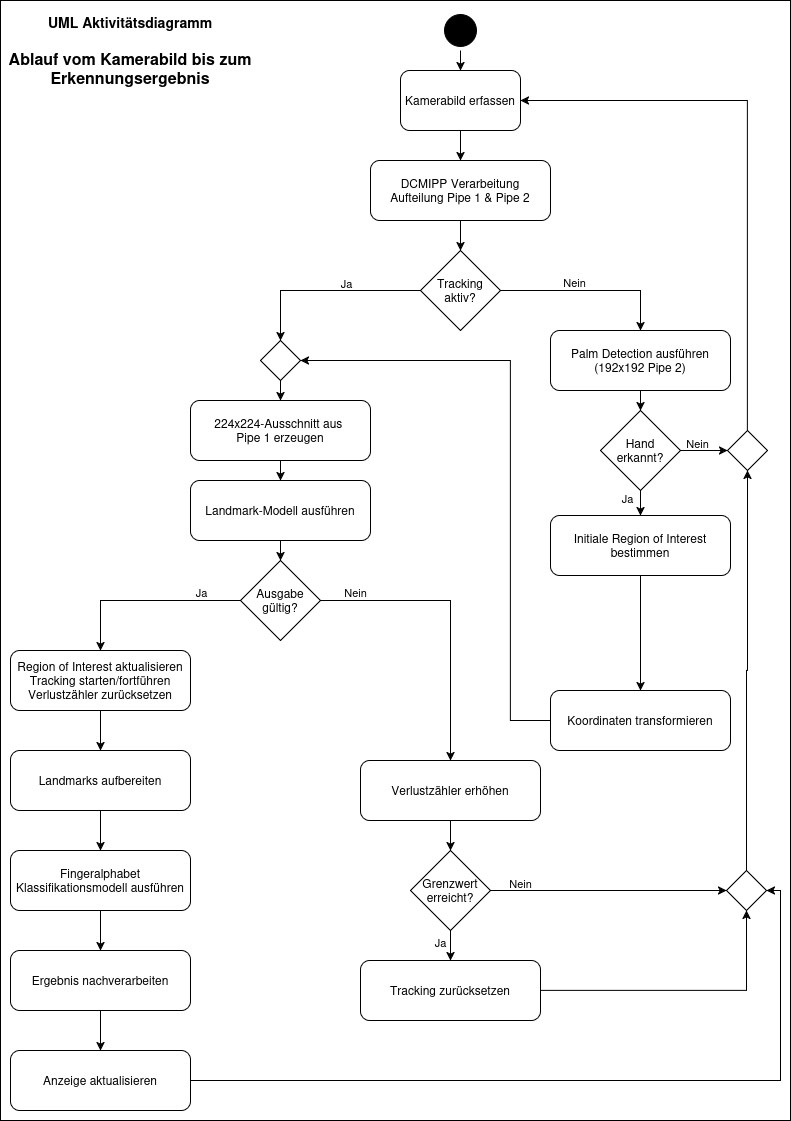
\includegraphics[width=1\textwidth]{material/figures/Aktivitätsdiagramm_ablauf.png}
    \caption{UML Aktivitätsdiagramm -- Ablauf vom Kamerabild bis zum Erkennungsergebnis}
    \label{fig:aktivitaetsdiagramm}
\end{figure}

Abbildung \ref{fig:aktivitaetsdiagramm} führt die zuvor beschriebenen Komponenten und Verarbeitungsschritte in einem gemeinsamen Ablauf zusammen. Nach der Erfassung wird das Kamerabild durch die DCMIPP verarbeitet und über Pipe 1 für die Display- und Landmark-Verarbeitung sowie über Pipe 2 für die Handdetektion bereitgestellt.

Ist noch kein Landmark-Tracking aktiv, wird zunächst die Handdetektion auf dem von Pipe 2 bereitgestellten Bild ausgeführt. Wird keine Hand erkannt, beginnt die Verarbeitung mit dem nächsten Kamerabild erneut. Bei einer erfolgreichen Erkennung wird eine initiale Region of Interest bestimmt und in das Koordinatensystem von Pipe 1 übertragen. Aus dem dort vorliegenden Displaybild wird anschließend ein 224×224 Pixel großer Ausschnitt für das Landmark-Modell erzeugt. Bei aktivem Tracking kann hierfür unmittelbar die anhand des vorherigen Bildes aktualisierte Region verwendet werden.

Nach der Ausführung des Landmark-Modells wird geprüft, ob eine gültige Modellausgabe vorliegt. Ist dies der Fall, wird die Region of Interest für den nächsten Durchlauf aktualisiert, das Tracking aktiviert beziehungsweise fortgeführt und der Verlustzähler zurückgesetzt. Anschließend werden die Landmark-Koordinaten entsprechend der in Abschnitt \ref{sec:ki-verarbeitungskette} beschriebenen KI-Verarbeitungskette aufbereitet und durch das Klassifikationsmodell einem Fingeralphabetzeichen zugeordnet. Das ermittelte Ergebnis wird nachverarbeitet und über die in Abschnitt \ref{sec:speicher-datenfluss} beschriebenen Anzeige- und Speicherbereiche für die grafische Ausgabe bereitgestellt.

Liegt keine gültige Landmark-Ausgabe vor, wird der Verlustzähler erhöht. Solange der festgelegte Grenzwert nicht erreicht ist, bleibt das Tracking aktiv und die Landmark-Erkennung wird mit dem nächsten Kamerabild erneut ausgeführt. Wird der Grenzwert erreicht, wird das Tracking zurückgesetzt, sodass im folgenden Durchlauf erneut eine Handdetektion auf dem vollständigen Eingabebild erfolgt.

Unabhängig vom jeweiligen Verarbeitungspfad kehrt der Ablauf anschließend zur Erfassung eines neuen Kamerabildes zurück. Dadurch entsteht ein kontinuierlicher Verarbeitungszyklus, der sowohl die erstmalige Lokalisierung einer Hand als auch deren anschließende Verfolgung und die wiederholte Klassifikation dargestellter Fingeralphabetzeichen ermöglicht.
